\documentclass[12pt]{article}
\usepackage{graphicx,hyperref}
\hypersetup{
colorlinks=true,
linkcolor=blue,
filecolor=magenta,
urlcolor=red,
}
%
% Title.
\title{Touchless Gesture Recognition Ideation and Simulation Report}
\author{Dimple Kochar , 16D070010 Harsh Deshpande , 16D070011 }


% begin the document.
\begin{document}

% make a title page.
\maketitle
\section{Simulation Results}
\subsection{Transmitter}
\subsection{Ultrasound Receiver}
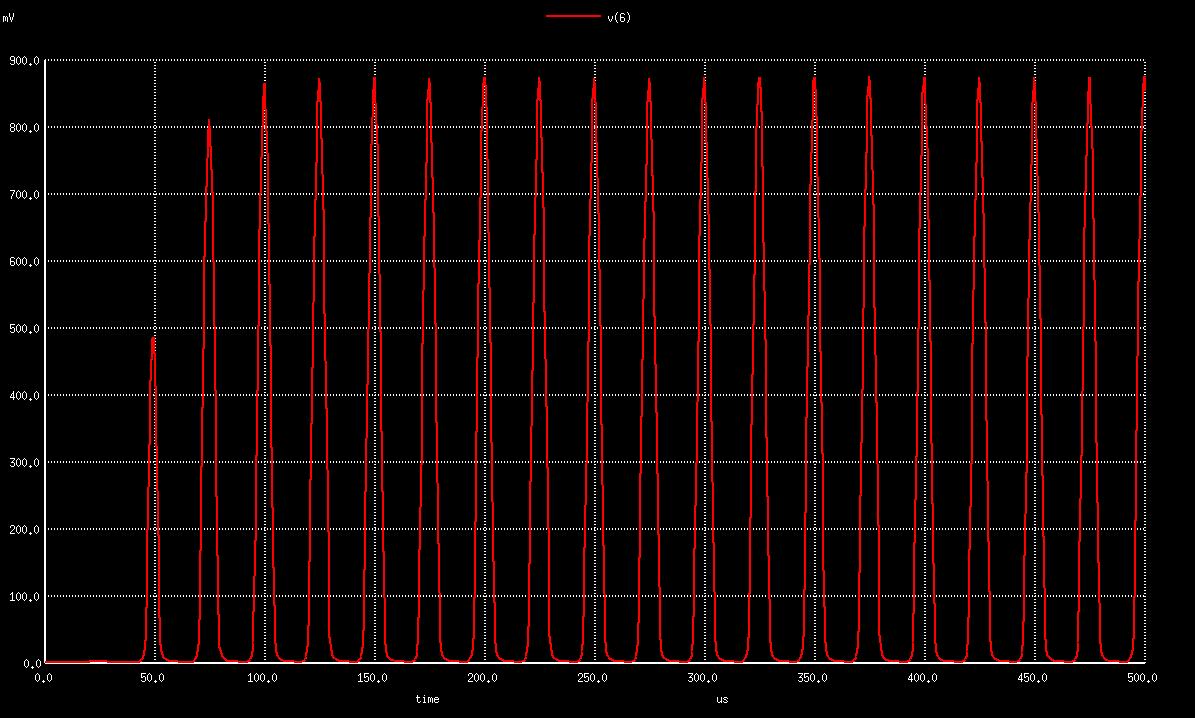
\includegraphics[scale=0.3]{rec.png} \\ \\
We assume that the receiver is getting a 5 mV, sinusoidal input, 40 KHz (from the transmitter), and simulate the circuit for receiver.  This signal is actually
received by an ultrasonic transducer which converts the sound wave to an electrical wave.
Due to attenuation, the signal received by the sensor is very weak. Thus, we use an amplifier and along with it a
filtering block. After that, we implement a peak detector which gives the peak value of its input. Comparator
gives a voltage high when the output of the peak detector
crosses a threshold level. Thus, when the peak detector detects
a sine wave at its input, the voltage of the comparator goes
high so as to indicate the reception of acoustic wave at the
receiver. When we increase the input signal amplitude from 5 to 6 mV, this is what we get-\\
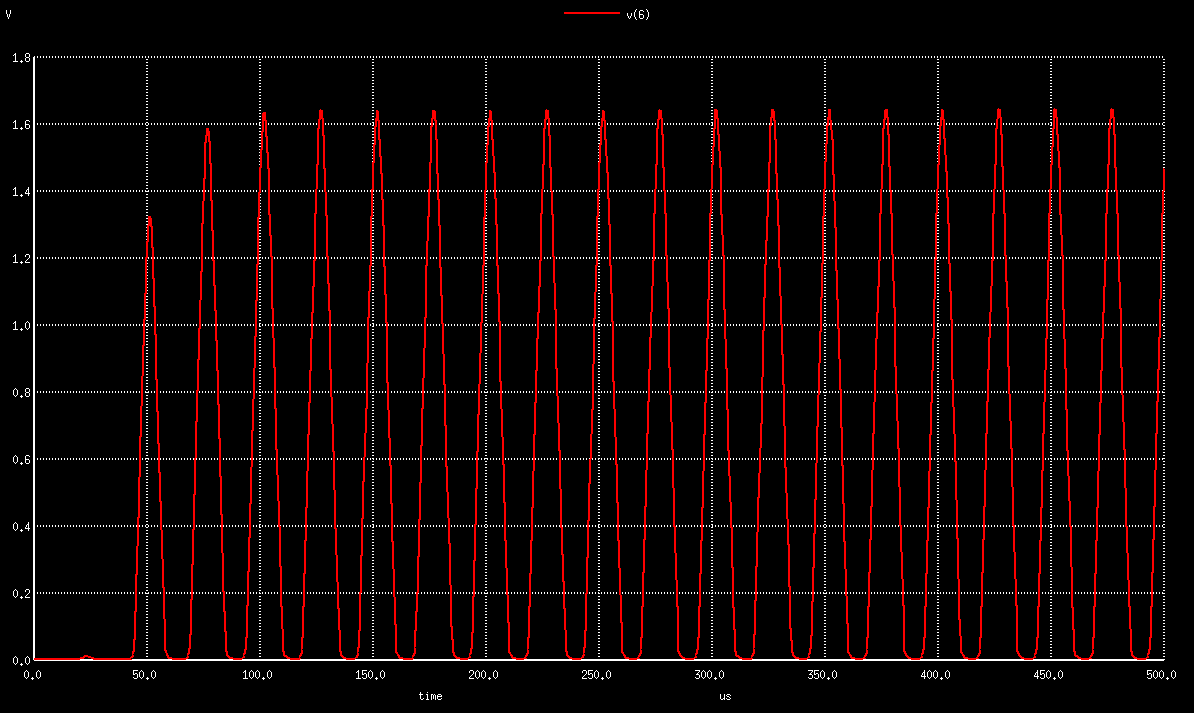
\includegraphics[scale=0.3]{r.png}\\ \\
That is, peak amplitude varies as signal varies.

\subsection{IV Receiver}
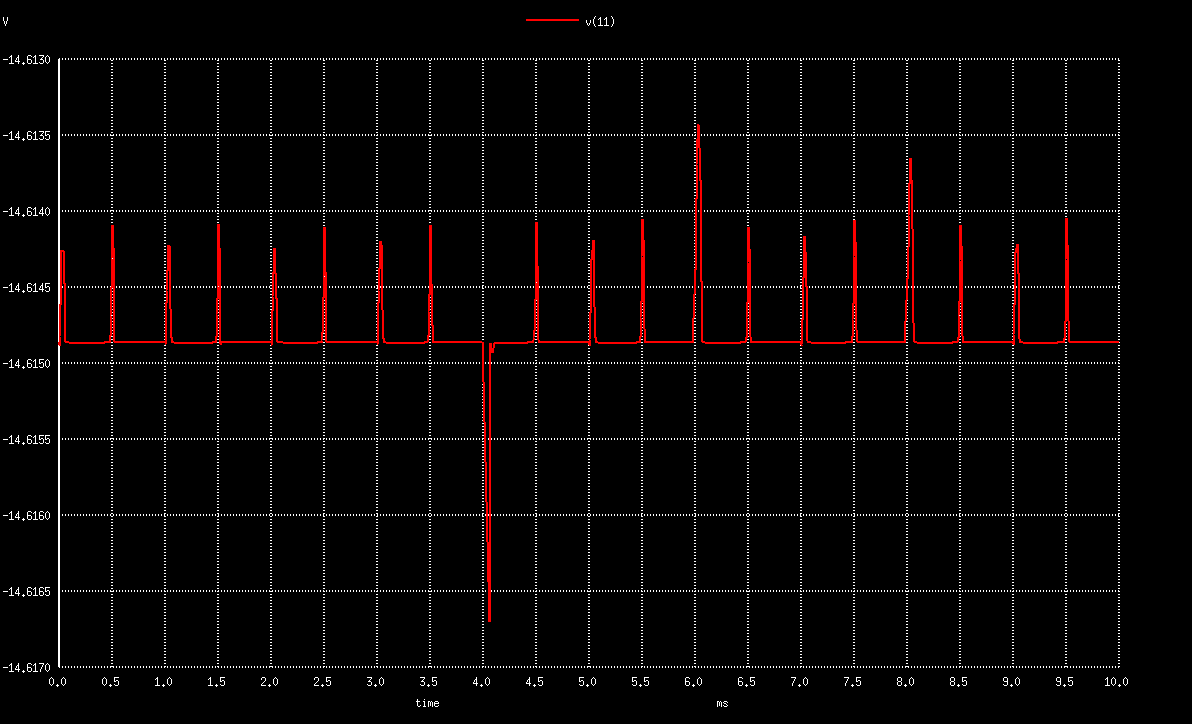
\includegraphics[scale=0.3]{ir.png} \\ \\
From the experiment, 'How Dark is Dark' that we did in lab 9, we simulate that circuit using a sinusoidal ac current source of amplitude 100 uA. \\
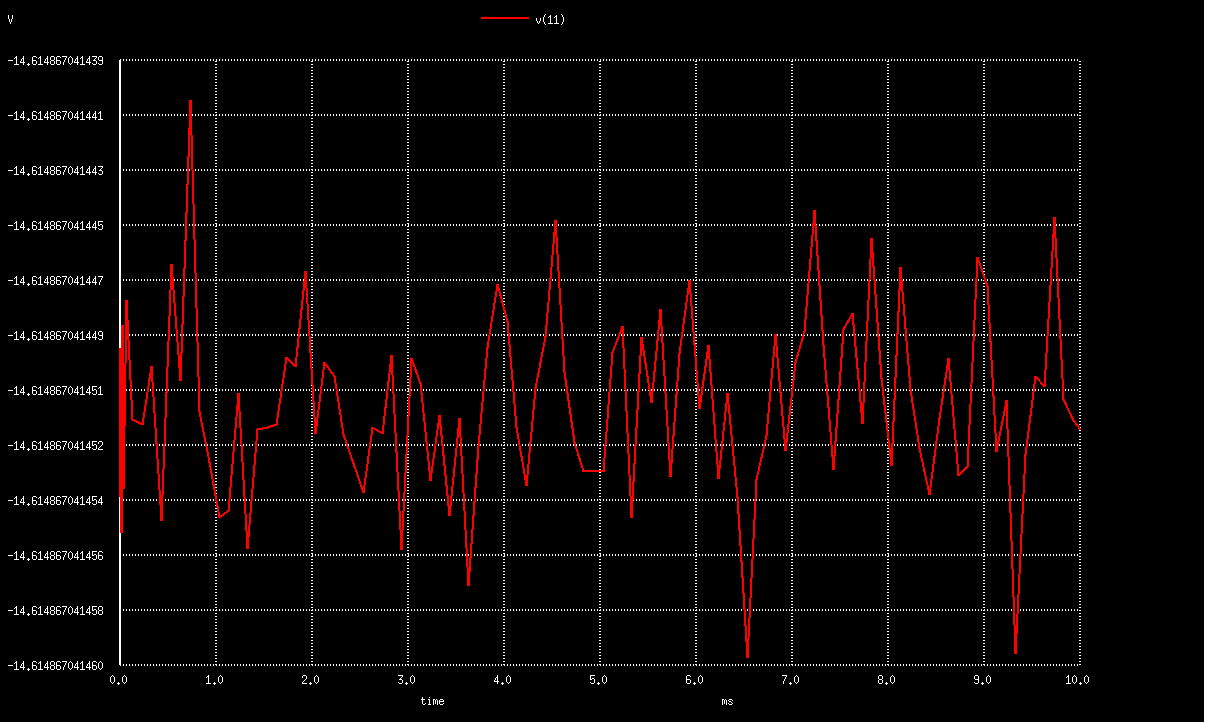
\includegraphics[scale=0.3]{irdc.png} \\ \\
We simulate that circuit using a dc current source of amplitude 100 uA. \\
\section{Observations and inferences} 
\subsection{Transmitter}
\subsection{Ultrasound Receiver}
\begin{tabular}{| c |c |} 


\hline 
Input Amplitude (in mV) & Output peak amplitude(in Volts) \\  
\hline  

2	&			0.00212	\\
3	&			0.00257	\\
4	&			0.0188\\
5	&			0.870	\\
6	&			1.635	\\
7	&			2.498	\\
8	&			4.754	\\
9	&			4.77	\\


\hline	% horizontal line.\\
\end{tabular}\\ \\
 Basically, saturates for >8mv which is okay because we don't expect that good a signal either.\\ \\
 The following graph gives the characteristics of this ultrasound receiver-\\
 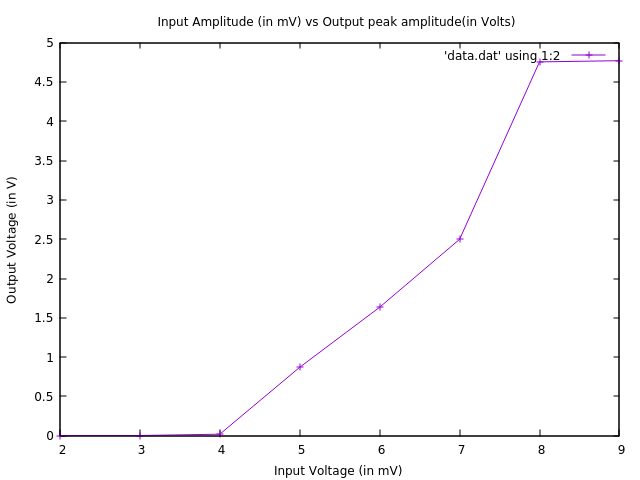
\includegraphics[scale=0.6]{g.png} \\ \\ 
 We can see that it functions pretty well as a receiver.

\subsection{IV Receiver}
On simulating it, we can see sharp peaks on detecting a photocurrent. These sharp peaks don't give a very large variation as much as the ultrasound detector on varying the input.
On simulating it with a dc current source, we get a constant voltage at the output.
\section{Appendix} 
\subsection{Code for Transmitter}
\begin{verbatim}

\end{verbatim}
\subsection{Code for Ultrasound Receiver}
\begin{verbatim}
 receiver
.include Diode_1N914.txt
.include lm324.txt
X1 11 12 1 0 13 LM324
X2 11 22 1 0 23 LM324
X3 11 32 1 0 33 LM324
X4 33 42 1 0 42 LM324
X5 51 11 1 0 53 LM324
vss 1 0 dc 12
r1 2 3 10k
c1 3 12 10n
r2 1 11 1k
r3 11 0 1k
c2 11 0 1u
c3 11 0 0.22u
r4 12 13 62k
r5 13 4 2.2k
r6 4 11 1k
c4 4 22 1n
c5 4 23 1n
r7 22 23 15.45k
c6 22 23 12p
r8 23 5 10k
c7 5 32 10n
r9 32 33 75k
d1 42 51 1N914
r10 51 0 61.6k
c8 51 0 2n
r11 53 6 12k
r12 6 0 10k
vin 2 0 sin(0 5m 40k) 
.tran 0.0001 0.5ms
.control
run
plot v(6)
.endc
.end
\end{verbatim}
\subsection{Code for IV Receiver}
\begin{verbatim}
receiver ir
.include ua741.txt
Is 1 2 sin(0 100u 1k)
vdc 1 0 dc 5
r1 2 3 10k
X1 0 3 5 6 7 ua741
vdd 5 0 dc 15
vss 6 0 dc -15
r2 5 7 100k
r3 7 8 1k
X2 0 8 5 6 11 ua741
r4 8 11 10k
.tran 0.0001 10ms
.control
run
plot v(11)
.endc
.end
\end{verbatim}
\subsection{Model File- Diode\_1N914.txt}
\begin{verbatim}
* Diode 1N914 SPICE Model Data

.MODEL 1N914 D (IS=6.2229E-9
+ N=1.9224
+ RS=.33636
+ IKF=42.843E-3
+ CJO=764.38E-15
+ M=.1001
+ VJ=9.9900
+ BV=100.14
+ IBV=.25951
+ TT=2.8854E-9)

*Developed by Wadhwani Electronics Lab
*Dept. of Electrical Engg.
*IIT Bombay
*January 09, 2015.
\end{verbatim}
\subsection{Model File- lm324.txt}
\begin{verbatim}
* LM324 OPERATIONAL AMPLIFIER "MACROMODEL" SUBCIRCUIT
* CREATED USING PARTS RELEASE 4.01 ON 09/08/89 AT 10:54
* (REV N/A)      SUPPLY VOLTAGE: 5V
* CONNECTIONS:   NON-INVERTING INPUT
*                | INVERTING INPUT
*                | | POSITIVE POWER SUPPLY
*                | | | NEGATIVE POWER SUPPLY
*                | | | | OUTPUT
*                | | | | |
.SUBCKT LM324    1 2 3 4 5
*
  C1   11 12 5.544E-12
  C2    6  7 20.00E-12
  DC    5 53 DX
  DE   54  5 DX
  DLP  90 91 DX
  DLN  92 90 DX
  DP    4  3 DX
  EGND 99  0 POLY(2) (3,0) (4,0) 0 .5 .5
  FB    7 99 POLY(5) VB VC VE VLP VLN 0 15.91E6 -20E6 20E6 20E6 -20E6
  GA    6  0 11 12 125.7E-6
  GCM   0  6 10 99 7.067E-9
  IEE   3 10 DC 10.04E-6
  HLIM 90  0 VLIM 1K
  Q1   11  2 13 QX
  Q2   12  1 14 QX
  R2    6  9 100.0E3
  RC1   4 11 7.957E3
  RC2   4 12 7.957E3
  RE1  13 10 2.773E3
  RE2  14 10 2.773E3
  REE  10 99 19.92E6
  RO1   8  5 50
  RO2   7 99 50
  RP    3  4 30.31E3
  VB    9  0 DC 0
  VC 3 53 DC 2.100
  VE   54  4 DC .6
  VLIM  7  8 DC 0
  VLP  91  0 DC 40
  VLN   0 92 DC 40
.MODEL DX D(IS=800.0E-18)
.MODEL QX PNP(IS=800.0E-18 BF=250)
.ENDS
\end{verbatim}
\subsection{Model File- ua741.txt}
\begin{verbatim}
*-----------------------------------------------------------------------------
*
* To use a subcircuit, the name must begin with 'X'.  For example:
* X1 1 2 3 4 5 ua741
*
* connections:   non-inverting input
*                |  inverting input
*                |  |  positive power supply
*                |  |  |  negative power supply
*                |  |  |  |  output
*                |  |  |  |  |
.subckt ua741    1  2  3  4  5
*
  c1   11 12 8.661E-12
  c2    6  7 30.00E-12
  dc    5 53 dx
  de   54  5 dx
  dlp  90 91 dx
  dln  92 90 dx
  dp    4  3 dx
  egnd 99  0 poly(2) (3,0) (4,0) 0 .5 .5
  fb    7 99 poly(5) vb vc ve vlp vln 0 10.61E6 -10E6 10E6 10E6 -10E6
  ga    6  0 11 12 188.5E-6
  gcm   0  6 10 99 5.961E-9
  iee  10  4 dc 15.16E-6
  hlim 90  0 vlim 1K
  q1   11  2 13 qx
  q2   12  1 14 qx
  r2    6  9 100.0E3
  rc1   3 11 5.305E3
  rc2   3 12 5.305E3
  re1  13 10 1.836E3
  re2  14 10 1.836E3
  ree  10 99 13.19E6
  ro1   8  5 50
  ro2   7 99 100
  rp    3  4 18.16E3
  vb    9  0 dc 0
  vc    3 53 dc 1
  ve   54  4 dc 1
  vlim  7  8 dc 0
  vlp  91  0 dc 40
  vln   0 92 dc 40
.model dx D(Is=800.0E-18 Rs=1)
.model qx NPN(Is=800.0E-18 Bf=93.75)
.ends
\end{verbatim}

\end{document}
